\documentclass[nooutcomes]{ximera}
%% handout
%% space
%% newpage
%% numbers
%% nooutcomes

%I added the commands here so that I would't have to keep looking them up
%\newcommand{\RR}{\mathbb R}
%\renewcommand{\d}{\,d}
%\newcommand{\dd}[2][]{\frac{d #1}{d #2}}
%\renewcommand{\l}{\ell}
%\newcommand{\ddx}{\frac{d}{dx}}
%\everymath{\displaystyle}
%\newcommand{\dfn}{\textbf}
%\newcommand{\eval}[1]{\bigg[ #1 \bigg]}

%\begin{image}
%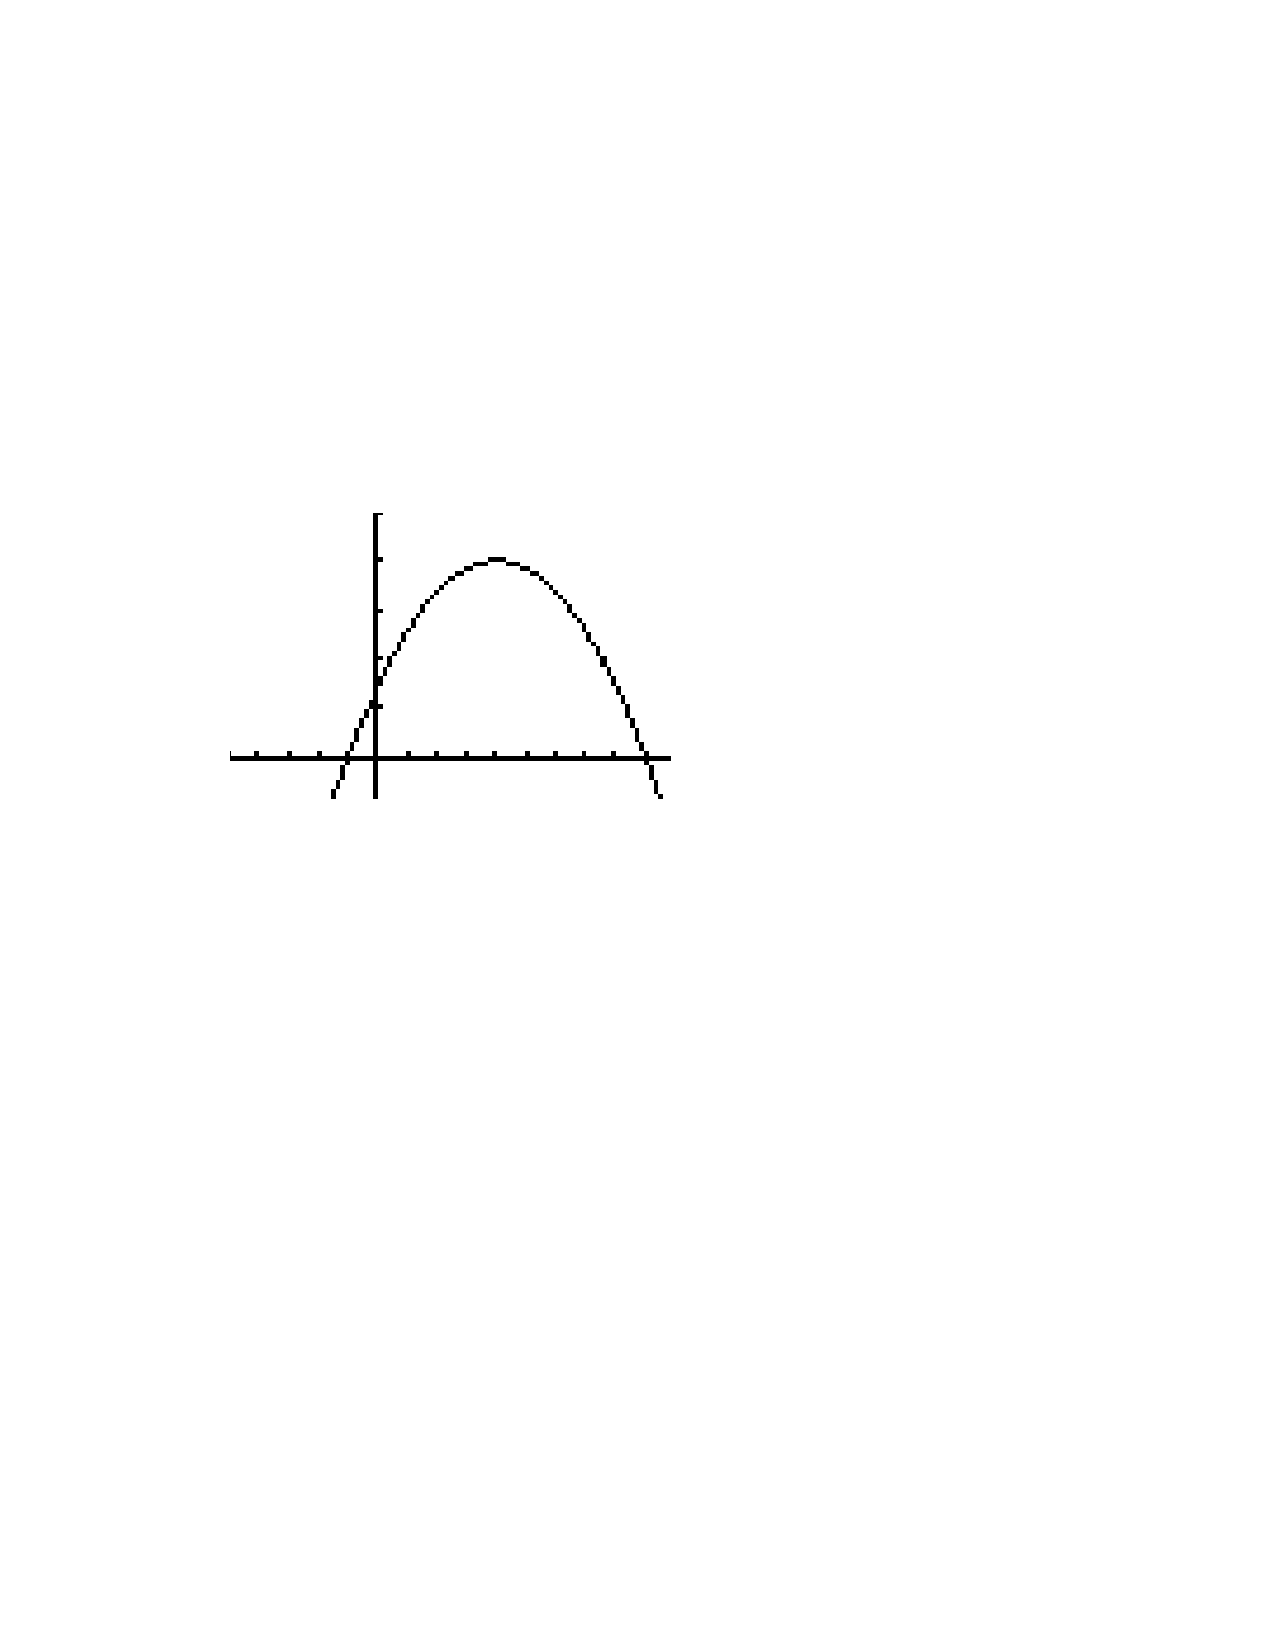
\includegraphics[trim= 170 420 250 180]{Figure1.pdf}
%\end{image}


\newcommand{\RR}{\mathbb R}
\renewcommand{\d}{\,d}
\newcommand{\dd}[2][]{\frac{d #1}{d #2}}
\renewcommand{\l}{\ell}
\newcommand{\ddx}{\frac{d}{dx}}
\newcommand{\dfn}{\textbf}
\newcommand{\eval}[1]{\bigg[ #1 \bigg]}

\usepackage{multicol}

\renewenvironment{freeResponse}{
\ifhandout\setbox0\vbox\bgroup\else
\begin{trivlist}\item[\hskip \labelsep\bfseries Solution:\hspace{2ex}]
\fi}
{\ifhandout\egroup\else
\end{trivlist}
\fi} %% we can turn off input when making a master document

\title{Recitation \#20 - 4.6 Mean Value Theorem (Solutions)}  

\begin{document}
\begin{abstract}		\end{abstract}
\maketitle

\section*{Warm up:} 
Heidi drives from her house in Columbus, OH to Tampa, FL for vacation.  Google maps says her driving distance is $1000$ miles.  The drive takes her $13$ hours.  The police send her a speeding ticket in the mail, saying she must have sped to arrive so quickly.  She is fighting the ticket, saying she just never stopped through the whole drive.  Can you prove she broke the $75$ mph speed limit at some point during her drive? 
		\begin{freeResponse}
		Let us define $s(t)$ to be the position function of Heidi after $t$ hours.  $s(t)$ will be continuous and differentiable because the location of a car is continuous and differentiable.  Heidi’s average speed for the whole trip is $\frac{1000}{13}\approx 76.9$ mph.  By the Mean Value Theorem, Heidi’s instantaneous speed was $76.9$ mph at some point of her trip: hence, she broke the $75$ mph speed limit.  
		\end{freeResponse}	
		
		
		

	
	
	
	
	

\section*{Group work:}



%problem 1
\begin{problem}
Verify that the given function satisfies the hypotheses of the Mean Value Theorem in the given interval.  Then algebraically find all numbers $c$ that satisfy the conclusion of the Mean Value Theorem.  Using the graph provided, label the point(s) $c$ and sketch the secant line and the tangent line at $c$
$$ f(x) = \frac{x}{x+2} \qquad \text{on } [1,4] $$.
	%\begin{image}
	%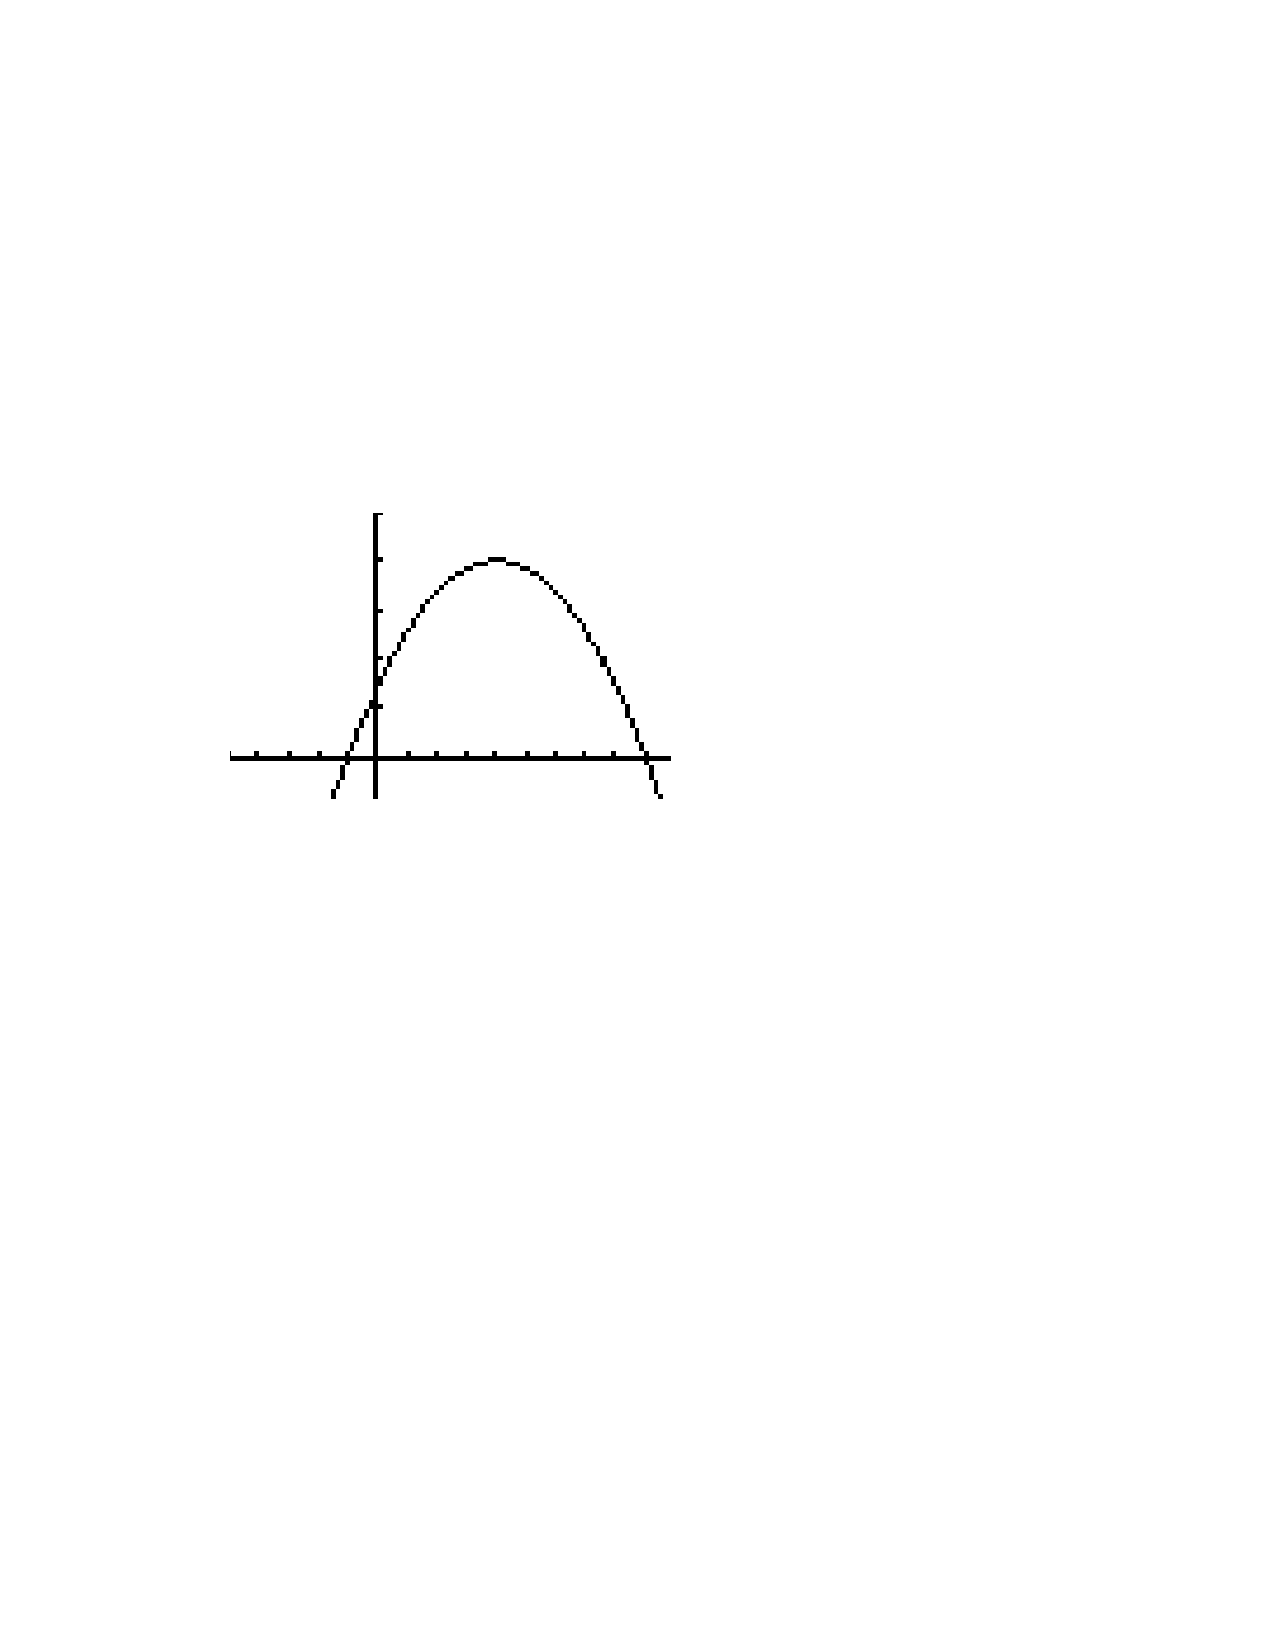
\includegraphics[trim= 170 420 250 180]{Figure1.pdf}
	%\end{image}
		\begin{freeResponse}
		The function $f(x) = \frac{x}{x+2}$ is continuous on $[1,4]$ and differentiable on $(1,4)$ since it is a rational function, and is therefore continuous and differentiable on its domain.  Therefore, $f$ satisfies the hypotheses of the Mean Value Theorem.  We have that
		$$ f'(x) = \frac{(x+2)(1) - x(1)}{(x+2)^2} = \frac{2}{(x+2)^2} $$
		$$ \frac{f(4) - f(1)}{4-1} = \frac{\frac{2}{3} - \frac{1}{3}}{3} = \frac{1}{9} $$
		So we are looking to find all points $c \in (1,4)$ which satisfy that $ f'(c) = \frac{1}{9} $.  So we solve:
		$$ \frac{2}{(c+2)^2} = \frac{1}{9} $$
		$$ (c+2)^2 = 18 $$
		$$ c = \sqrt{18} - 2 = 3\sqrt{2} - 2 $$
		Note that we omitted $-\sqrt{18} - 2$ above because it is not in the interval $(1,4)$.  Therefore, $c = 3\sqrt{2} - 2$.
		
		%\begin{image}
		%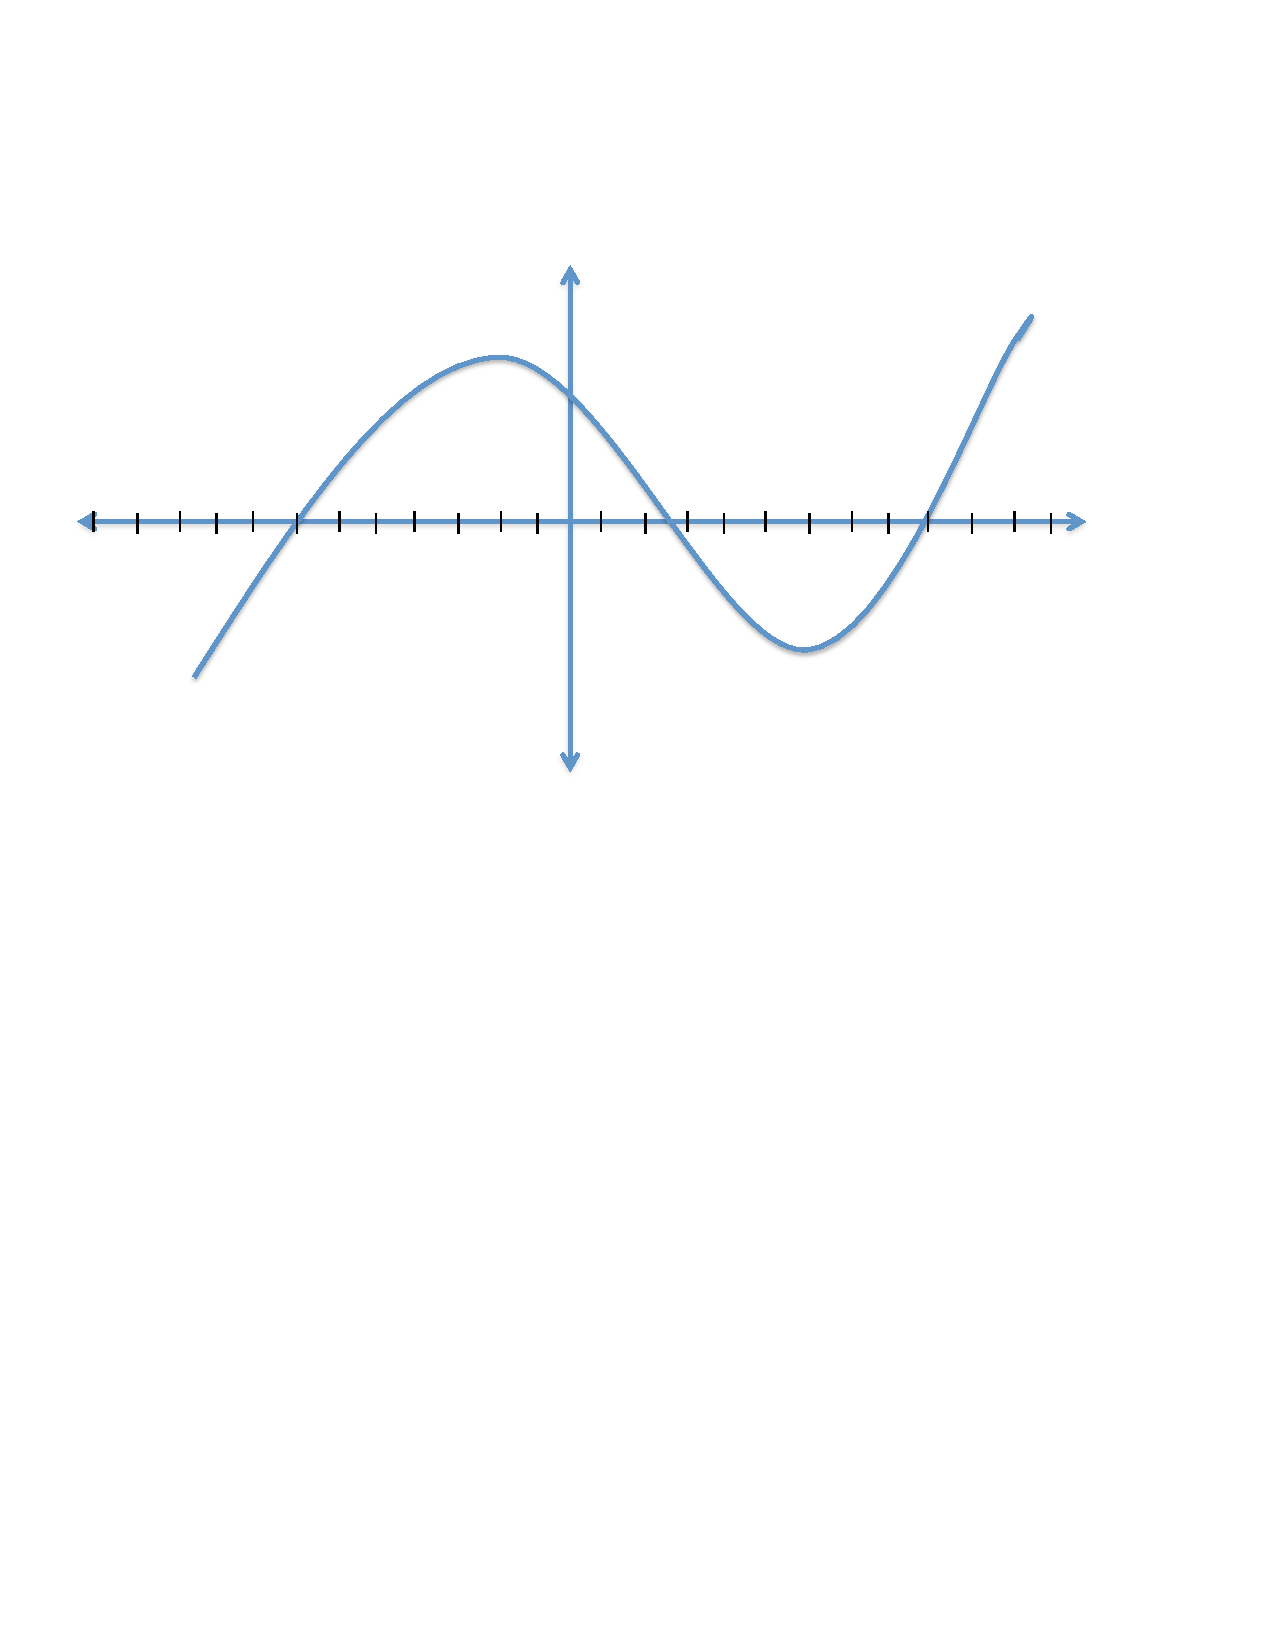
\includegraphics[trim= 170 420 250 180]{Figure2.pdf}
		%\end{image}
		\end{freeResponse}
		
		
\end{problem}
















%problem 2
\begin{problem}

		\begin{freeResponse}
		
		\end{freeResponse}
		
		
		

\end{problem}
	
	
	
	
	
	
	
	
			
			

%problem 3
\begin{problem}

		\begin{freeResponse}
			
		\end{freeResponse}
			
			
		
\end{problem}











%problem 4
\begin{problem}

		\begin{freeResponse}

		\end{freeResponse}
			
			
	
\end{problem}






	
	
	
	
	
	
	
	
	

	










								
				
				
	














\end{document} 


















